\documentclass[a4paper, 10pt]{article}
\usepackage[left=2cm, right =2cm, top=2cm, bottom=3cm]{geometry}
% Useful packages
\usepackage{amsmath,physics, amssymb}
\usepackage{graphicx}
\usepackage[colorlinks=true, allcolors=blue]{hyperref}
\usepackage{color}
\newcommand{\blue}[1]{\textcolor{blue}{#1}}
\newcommand{\red}[1]{\textcolor{red}{#1}}
\usepackage{soul, ulem, todonotes}
%\usepackage{mathptmx}

\usepackage[capitalise]{cleveref}
%\usepackage[backend=bibtex, citestyle=numeric-comp, sorting=none, url =false]{biblatex}
\usepackage[backend=biber, style=numeric]{biblatex}
\addbibresource[]{discussion.bib}  
% Include bibliography from discussion.bib
% The bibliography will be printed at the end using \printbibliography{}
\setcounter{tocdepth}{2}

% Sans modern font
%\usepackage{sansmath}
%\renewcommand{\familydefault}{\sfdefault}
%\sansmath

\title{Impurity induced flat-band discrete time crystal}
\usepackage{authblk}
\author[1]{Mahbub Rahaman}
\author[1]{Sayan Choudhury}
\affil[1]{\small Harish-Chandra Research Institute, HBNI, Chhatnag Road, Jhunsi, Praygraj, UP - 211019, India}
\date{}
\begin{document}
\maketitle
%\tableofcontents
%\newpage

\section{The Model and Dynamics}
We study a flat-band protocol generated by a carefully designed two-frequency periodic drive. The system’s time-dependent Hamiltonian is given by
\begin{align}
    \hat{\mathcal{H}}_{\text{total}}(t) &=  \hat{\mathcal{H}}_0(t) + \hat{\mathcal{H}}_1(t)  + \hat{\mathcal{H}}_2(t), \\
    \hat{\mathcal{H}}_0(t) &= J(t)\sum_{j} \hat{\sigma}_j^z \hat{\sigma}_{j+1}^z, \quad J(t) = J\, \mathrm{sgn}[\cos(\omega t)], \\
    \hat{\mathcal{H}}_1(t) &= g(t)\sum_{j}\hat{\sigma}_j^x, \quad g(t) = g\, \mathrm{sgn}[\cos(2 \omega t)], \\
    \hat{\mathcal{H}}_2(t) &=
    \begin{cases}
        0, & 0 < t \leq \frac{T}{2}, \\
        \lambda_s \sum_{j}\hat{\sigma}_j^x, & \frac{T}{2} < t \leq T,
    \end{cases}
\end{align}
where $\hat{\sigma}_j^{x,y,z}$ denote the Pauli matrices at site $j$, $J$ is the Ising interaction strength, $g$ is the transverse field amplitude, and $\lambda_s$ is the amplitude of the secondary drive, chosen such that $\lambda_s \frac{T}{2} = \frac{\pi}{2}$. The primary drive has period $T = 2\pi/\omega$. The system is subjected to two square pulse drives at frequencies $\omega$ and $2\omega$. The first term, $\hat{\mathcal{H}}_0(t)$, describes a periodically modulated Ising interaction, while the second term, $\hat{\mathcal{H}}_1(t)$, represents a periodically driven transverse field. Together, these drives establish the flat-band protocol, resulting in completely localized states (CLS). The third term, $\hat{\mathcal{H}}_2(t)$, implements a global spin-flip operation during the second half of each period, which induces a period-doubled response and ultimately leads to the emergence of a discrete time crystal (DTC) phase.

The Floquet Hamiltonian, $\hat{\mathcal{H}}_F$, is defined via the relation $\hat{U}(T,0) = e^{-i \hat{\mathcal{H}}_F T}$, where $\hat{U}(T,0)$ is the time-evolution operator over one period $T$:
\begin{align}
    \hat{\mathcal{H}}_F = \frac{i}{T} \ln[\hat{U}(T,0)].
\end{align}

Applying the Suzuki-Trotter decomposition and Zassenhaus’ formula, the propagator can be written as
\begin{align}
    \hat{U}(T,0) =& \exp\left(-i \lambda_s \frac{T}{2} \sum_{j}\hat{\sigma}_j^x\right)
    \exp\left(i g \frac{T}{4} \sum_{j}\hat{\sigma}_j^x\right)
    \exp\left(-i g \frac{T}{4} \sum_{j}\hat{\sigma}_j^x\right)\exp\left(i J \frac{T}{2} \sum_{j} \hat{\sigma}_j^z \hat{\sigma}_{j+1}^z\right)\nonumber\\
    &\hspace{4cm}\exp\left(i g \frac{T}{4} \sum_{j}\hat{\sigma}_j^x\right)\exp\left(-i g \frac{T}{4} \sum_{j}\hat{\sigma}_j^x\right)\exp\left(-i J \frac{T}{2} \sum_{j} \hat{\sigma}_j^z \hat{\sigma}_{j+1}^z\right).
\end{align}
The Floquet Hamiltonian can be computed numerically by evaluating the logarithm of the propagator, and its quasienergy spectrum is obtained by diagonalizing $\hat{\mathcal{H}}_F$.

\subsection{Flat-Band Protocol and Emergent CLS}
When the spin-flip operation $\hat{\mathcal{H}}_2(t)$ is ignored, the system is governed by a reduced Hamiltonian that yields a flat band in its quasienergy spectrum:
\begin{align}
    \hat{\mathcal{H}}_{\text{eff}}(t) = \hat{\mathcal{H}}_0(t) + \hat{\mathcal{H}}_1(t).
\end{align}
The corresponding Floquet Hamiltonian is defined via $\hat{U}_{\text{eff}}(T,0) = e^{-i \hat{\mathcal{H}}_{\text{eff},F} T}$, where the propagator is after neglecting higher-order commutators through the Suzuki-Trotter decomposition and Zassenhaus’ formula, the propagator simplifies to
\begin{align}
    \hat{U}_{\text{eff}}(T,0) =& 
        \exp\left(i g \frac{T}{4} \sum_{j}\hat{\sigma}_j^x\right)
        \exp\left(-i g \frac{T}{4} \sum_{j}\hat{\sigma}_j^x\right)\exp\left(i J \frac{T}{2} \sum_{j} \hat{\sigma}_j^z \hat{\sigma}_{j+1}^z\right)\nonumber\\
        &\hspace{4cm}\exp\left(i g \frac{T}{4} \sum_{j}\hat{\sigma}_j^x\right)\exp\left(-i g \frac{T}{4} \sum_{j}\hat{\sigma}_j^x\right)\exp\left(-i J \frac{T}{2} \sum_{j} \hat{\sigma}_j^z \hat{\sigma}_{j+1}^z\right)\nonumber\\
        =& \mathbb{I}.
\end{align}
Consequently, $\hat{\mathcal{H}}_{\text{eff},F} = 0$, signifying a perfectly flat quasienergy spectrum. This analytical result is corroborated by numerical simulations, as illustrated in \cref{fig:drive}.

\begin{figure}[h!]
    \centering
    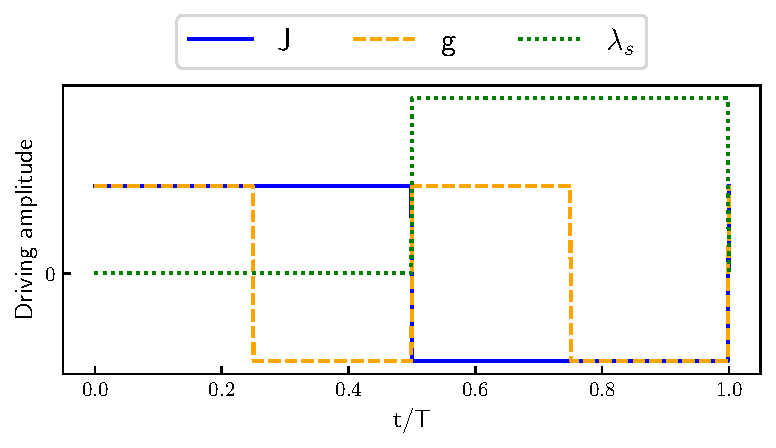
\includegraphics[width=0.45\textwidth]{figs/drive.pdf}
    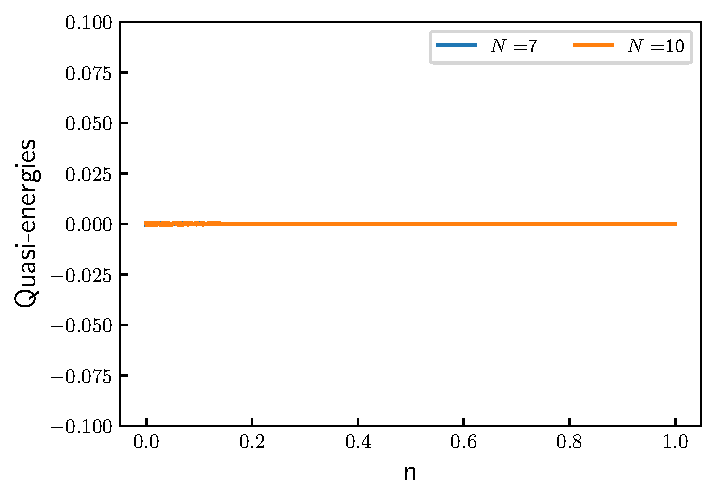
\includegraphics[width=0.4\textwidth]{figs/pure_flatband.pdf}
    \caption{Schematic representation of the two-frequency drive protocol. The first drive, $\hat{\mathcal{H}}_0(t)$, is a square pulse with period $T$, while the second drive, $\hat{\mathcal{H}}_1(t)$, is a square pulse with period $T/2$. The third component, $\hat{\mathcal{H}}_2(t)$, implements a spin-flip operation during the latter half of each period. The right panel displays the quasienergy spectrum of the effective Floquet Hamiltonian (flat-band only), $\hat{\mathcal{H}}_{\text{eff},F}$, which exhibits a perfectly flat band structure. Parameters: $J=0.18$, $g=J/2$, system sizes $L=7, 10$.}
    \label{fig:drive}
\end{figure}

\subsection{Impurity in the Flat-Band Protocol and Emergent DTC}
The inclusion of the spin-flip operation $\hat{\mathcal{H}}_2(t)$ introduces an impurity into the flat-band protocol, flipping all spins during the second half of each period and thereby inducing a period-doubled response in the system's dynamics. The complete Floquet Hamiltonian, $\hat{\mathcal{H}}_F$, encompasses all three components of the time-dependent Hamiltonian, with the spin-flip term perturbing the perfectly flat quasienergy spectrum and resulting in a nontrivial band structure.

To investigate the impact of this impurity, we numerically compute the magnetization dynamics, initializing the system in a fully polarized state, $\ket{\psi(0)} = \ket{\uparrow \uparrow \uparrow \ldots \uparrow}$. The magnetization at site $j$ evolves as
\begin{align}
    m_j(t) = \bra{\psi(t)} \hat{\sigma}_j^z \ket{\psi(t)},
\end{align}
where $\ket{\psi(t)} = \hat{U}(t,0) \ket{\psi(0)}$. The resulting magnetization exhibits oscillations with period $2T$, indicative of discrete time crystal (DTC) behavior. However, the impurity term undermines the stability of the DTC phase, leading to a gradual decay of these oscillations, as shown in Fig.~\ref{figs:impure_flatband_dtc}.
\begin{figure}[h!]
    \centering
    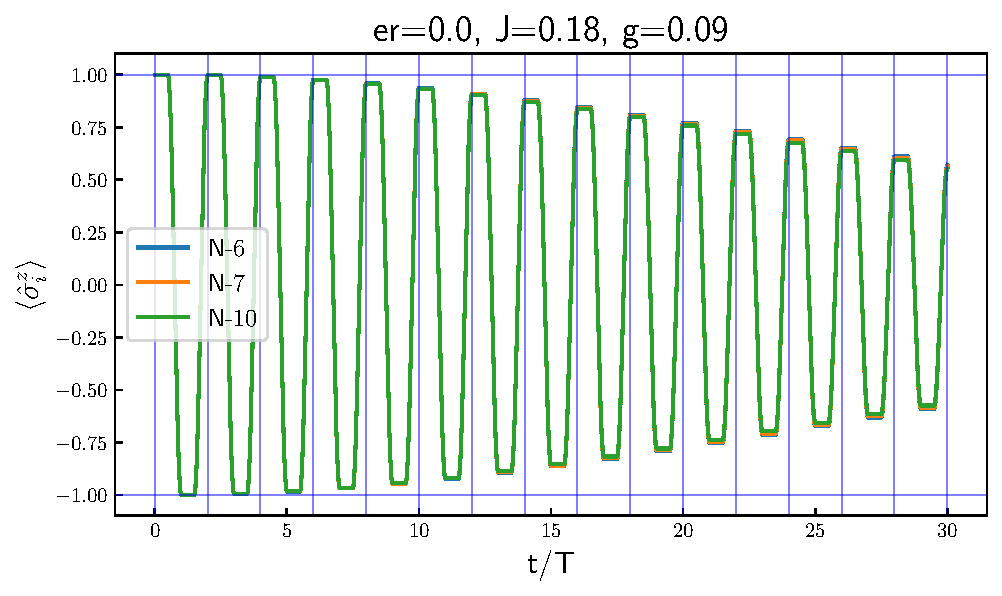
\includegraphics[width=0.45\textwidth]{figs/mag_er0.0_J0.18_g0.09.pdf}
    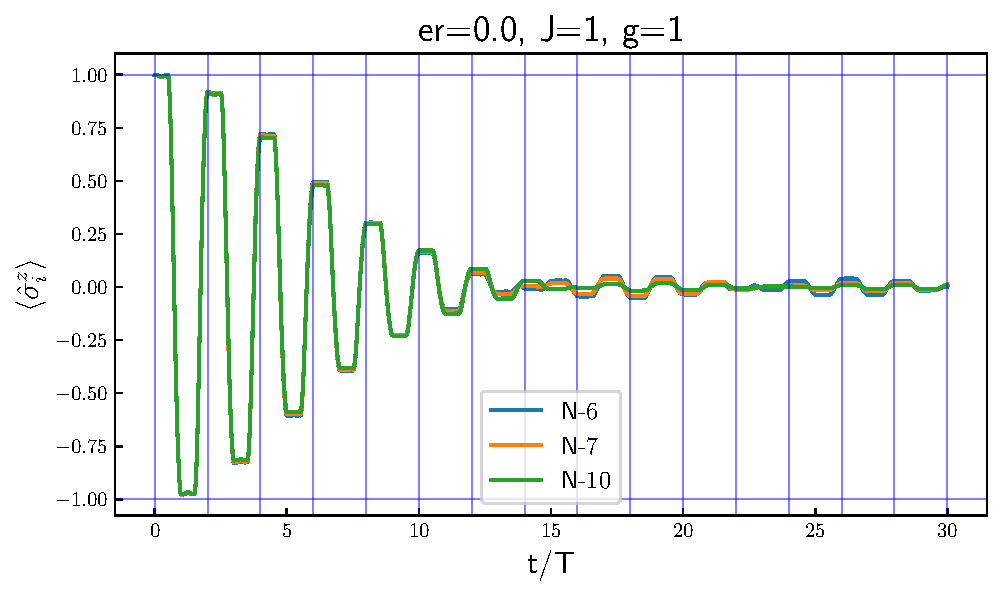
\includegraphics[width=0.45\textwidth]{figs/mag_er0.0_J1_g1.pdf}
    \caption{Time evolution of the magnetization for a system initialized in the fully polarized state, $\ket{\psi(0)} = \ket{\uparrow \uparrow \uparrow \ldots \uparrow}$. Left: Magnetization dynamics for moderate interaction strength ($J=0.18$, $g=J/2$), showing gradual decay of period-doubled oscillations due to the impurity term. Right: Stronger interactions ($J=1$, $g=1$) result in more rapid decay and faster loss of DTC order. In both cases, the impurity-induced spin-flip operation breaks the flatness of the quasienergy spectrum, leading to relaxation and dephasing.}
    \label{figs:impure_flatband_dtc}
\end{figure}

This decay is attributable to the nonzero bandwidth introduced by the spin-flip operation, which manifests as dephasing and relaxation processes. The quasienergy spectrum of the full Floquet Hamiltonian, $\hat{\mathcal{H}}_F$, is presented in Fig.~\ref{figs:impure_flatband_qe}, illustrating the departure from the ideal flat-band structure.
\begin{figure}[h!]
    \centering
    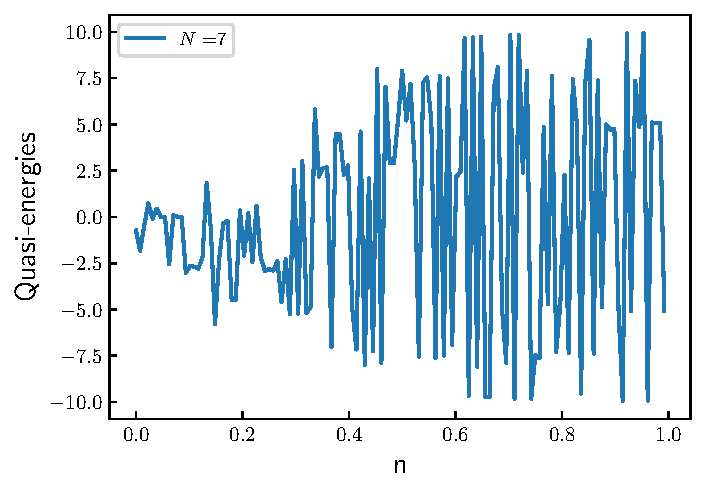
\includegraphics[width=0.45\textwidth]{figs/impure_flatband_qe.pdf}
    \caption{Quasienergy spectrum of the full Floquet Hamiltonian, $\hat{\mathcal{H}}_F$, including the impurity term $\hat{\mathcal{H}}_2(t)$. Parameters: $J=0.18$, $g=J/2$, system size $L=7$, drive frequency $\omega=20$. The impurity induces a nonzero bandwidth within the range $\in[-\omega/2 , \omega/2]$, thereby breaking the perfect flatness of the quasienergy spectrum.}
    \label{figs:impure_flatband_qe}
\end{figure}

\subsection{Flatband DTC}
The combination of the flat-band protocol with the impurity term $\hat{\mathcal{H}}_2(t)$ gives rise to a discrete time crystal (DTC) phase, characterized by period-doubled oscillations in the magnetization. The spin-flip operation perturbs the ideal flatness of the quasienergy spectrum, introducing a finite bandwidth that facilitates dephasing and relaxation. The stability of the DTC phase is governed by the interplay between the transverse field in flatband protocol and spin flip operator. To improve the robustness of the DTC phase, we consider an alternative scheme in which the spin-spin Ising interactions and transverse fields are oriented along different axes, resulting in a modified Hamiltonian:

\begin{align}
    \hat{\mathcal{H}}_{\text{total}}(t) &=  \hat{\mathcal{H}}_0(t) + \hat{\mathcal{H}}_1(t)  + \hat{\mathcal{H}}_2(t), \\
    \hat{\mathcal{H}}_0(t) &= J(t)\sum_{j} \hat{\sigma}_j^x \hat{\sigma}_{j+1}^x, \quad J(t) = J\, \mathrm{sgn}[\cos(\omega t)], \\
    \hat{\mathcal{H}}_1(t) &= g(t)\sum_{j}\hat{\sigma}_j^z, \quad g(t) = g\, \mathrm{sgn}[\cos(2 \omega t)], \\
    \hat{\mathcal{H}}_2(t) &=
    \begin{cases}
        0, & 0 < t \leq \frac{T}{2}, \\
        \lambda_s (1- \epsilon)\sum_{j}\hat{\sigma}_j^x, & \frac{T}{2} < t \leq T,
    \end{cases}
\end{align}
where the spin-flip operation is now implemented along the $x$-direction. This modification is designed to minimize additional spin rotation errors and enhance the stability of the DTC phase.

We numerically investigate the magnetization dynamics for this modified Hamiltonian, initializing the system in the fully polarized state $\ket{\psi(0)} = \ket{\uparrow \uparrow \uparrow \ldots \uparrow}$ and considering the ideal protocol with zero rotational error ($\epsilon = 0$). The results, presented in Fig.~\ref{figs:clean_flatband_dtc}, reveal robust period-doubled oscillations with negligible melting rate, indicating that the choice of interaction and transverse field directions is crucial for stabilizing the DTC phase against dephasing and relaxation.

\begin{figure}[h!]
    \centering
    
\includegraphics[height=5cm]{figs/DTC_mag_inset_er=0.0_J=0.18_g=0.09.pdf}
    \caption{}
    \label{figs:clean_flatband_dtc}
\end{figure}

\subsubsection{Impact of Rotational Error}
Nevertheless, the introduction of a small rotational error ($\epsilon = 0.03$) in the spin-flip operation leads to a gradual decay of the DTC phase, as shown in Fig.~\ref{figs:clean_flatband_dtc_er}. These findings suggest that, while the modified Hamiltonian enhances the stability of the DTC phase, it remains susceptible to imperfections in the driving protocol.

\begin{figure}[h!]
    \centering
    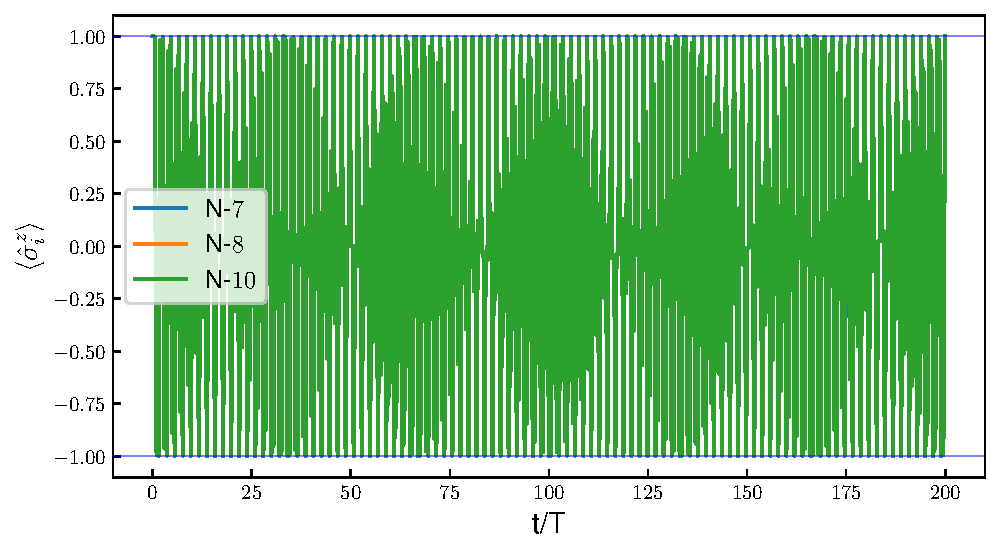
\includegraphics[width=0.45\textwidth]{figs/DTC_mag_inset_er=0.03_J=0.18_g=0.09.pdf}
    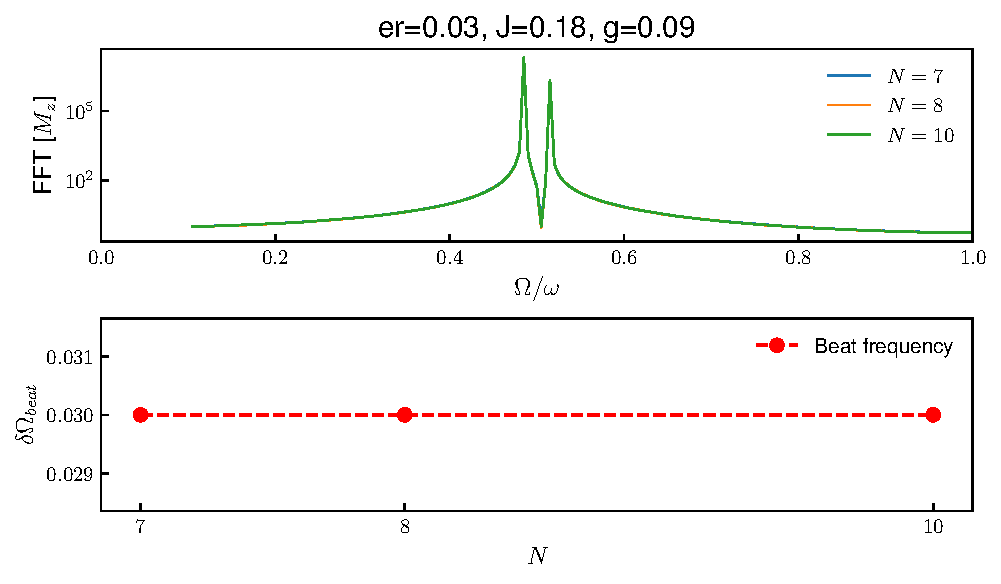
\includegraphics[width=0.45\textwidth]{figs/DTC_mag_fft_inset_er=0.03_J=0.18_g=0.09.pdf}\\
    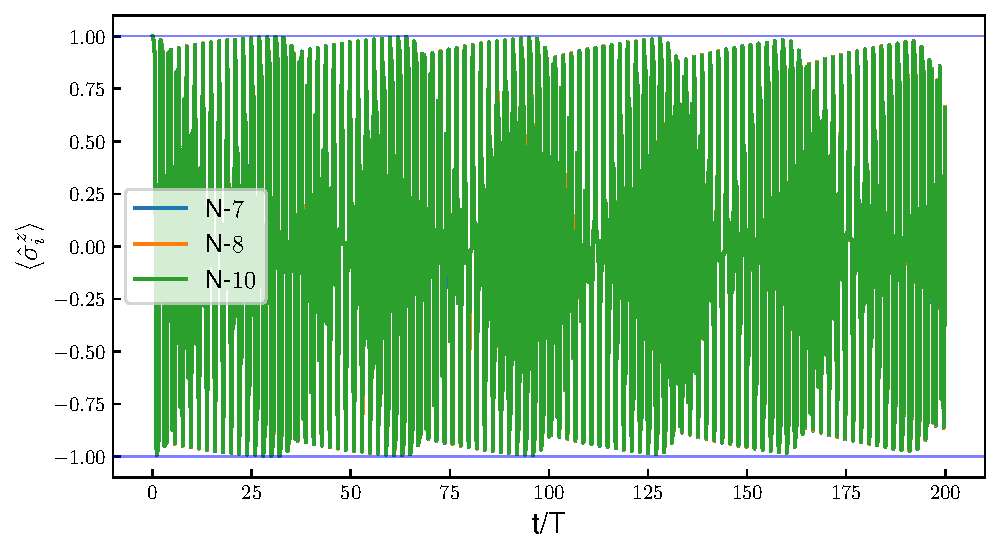
\includegraphics[width=0.45\textwidth]{figs/DTC_mag_inset_er=0.03_J=1_g=1.pdf}
    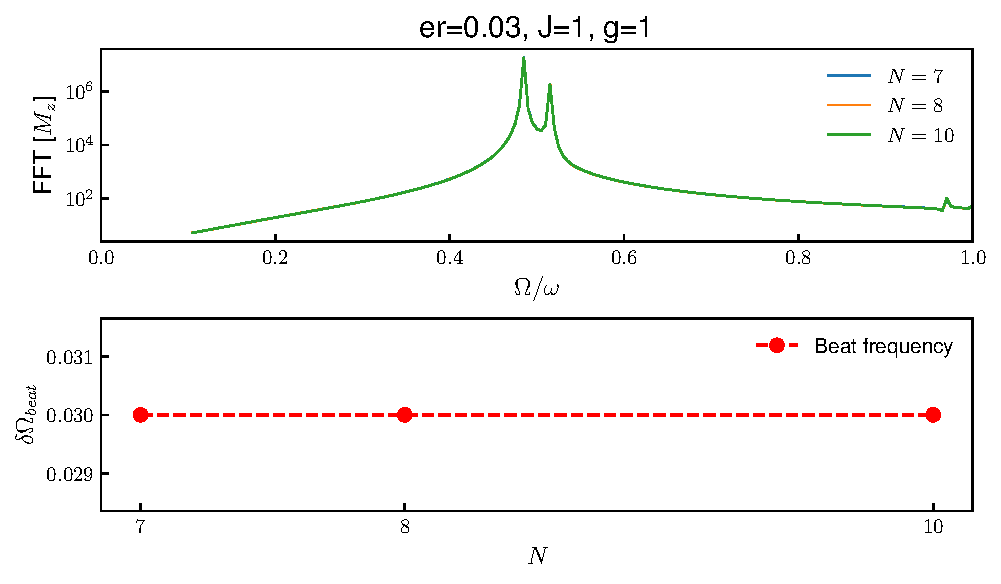
\includegraphics[width=0.45\textwidth]{figs/DTC_mag_fft_inset_er=0.03_J=1_g=1.pdf}
    \caption{Time evolution of the magnetization for a system initialized in the fully polarized state, $\ket{\psi(0)} = \ket{\uparrow \uparrow \uparrow \ldots \uparrow}$, with a small rotational error ($\epsilon = 0.03$) in the spin-flip operation. Top panels: Moderate interaction strength ($J=0.18$, $g=J/2$) exhibits gradual decay of period-doubled oscillations due to the impurity term. Bottom panels: Stronger interactions ($J=1$, $g=1$) result in more rapid decay and accelerated loss of DTC order. The right panels display the corresponding Fourier transforms, highlighting the emergence of subharmonic peaks at $\omega/2$.}
    \label{figs:clean_flatband_dtc_er}
\end{figure}



\end{document}